 \section{Hardware}
%metatekst til hardware
Dette afsnit skal være med til at dokumentere hardwaren i systemet \textit{the cell collector}, derfor indeholder afsnittet beskrivelser af systemets fysiske dele og deres funktionalitet. De fysiske deles specifikationer er uddybet og beskrevet i dette dokument. Der er begrundelser og argumenter for hvorfor de brugte komponenter er valgt. Desuden er der også et teori afsnit til hver komponent, for at dokumentere den forskning der er lavet.

\subsection{Læsevejledning til hardware}
%læsevejledning
Da dette afsnit er en udspecificering af hvilke specifikationer hardware komponenterne består af, afsnittet ligger sig tæt op af kravspecifikationen. Da det er kravene i kravspecifikationen, der ligger til grunde for de valgte hardware dele. I afsnittet findes der forskellige diagrammer der er med til at beskrive opbygningen, og kommunikationen af delene. Til hvert diagram vil der være en kort beskrivelse af hvad det indeholder. Hvert afsnit indeholder funktionalitet, specifikationer omkring det enkle komponent, samt begrundelser og argumentationer for valgende, i den skrevne rækkefølge. Til sidst er der et teori afsnit til hver komponent, hvilket kan springes over hvis viden her om allerede er etableret. Afsnittene kan godt læses i dele, men for en komplet forståelse bør afsnittene læses i rækkefølge. 

%Det gamle afsnit, måske skal det være i et leverandør afsnit 
% Dette afsnit indeholder den nødvendige viden hardware delene i systemet Denne blok beskriver forbindelserne mellem diverse hardware med et internal block definition diagram. Dette diagram er med til at sikre at delene kan kommunikere sammen, uden unødvendige adaptere og omformere. Yderligere er der beskrevet hvordan information søgning, og viden er fundet omkring komponenterne. Primær kan det siges at hardware delene er fundet på Ebay.com(kilder til de konkrete sider?(måske under hvert produkt?)), for at hold budgettet i bund. Den manglende datablade og lidt tvivlsomme kvalitet er accepteret, da dette projekt først og fremmest er  ”\textit{proof of concept}” projekt.
\subsection{Leverandør af produkter}
Når der skal vælges leverandør til et produkt er det vigtigt, at de er pålidelige. Da delene skal kunne leveres i hele produktets levetid. Specielt hvis produktet kræver en stor dokumentation og godkendelse, som for eksempel medicinsk udstyr. Når produktet skal sættes i produktion bør der være flere leverandører, som kan leverer det samme produkt. Det er vigtigt for, at dokumentationen ikke skal ændres, fordi at en lille del af produktet er udgået af underleverandørens portefølje.
Til systemet \textit{The cell collector}, har budgettet gjort stort præg af hvilke leverandører der er valgt. Primært er de fleste dele fundet på Ebay, for netop at holde budgettet og dermed priserne i bund. Dette medfører selvfølgelig at kvaliteten er nedprioriteret, som et kompromis er kameraet(\ref{subsec:Kamera}) i projektet købt ved Farnell. Farnell er en mere pålidelig forhandler end Ebay. At produkterne er købt på Ebay, vil medfører at der vil komme ændringer af dokumentation for  at hæve kvaliteten på produktet i fremtiden. Ydermere er generelle ikke elektroniske komponenter købt ved \citep{Mikrolab}, herunder slanger og beholdere. 

     
%gamle afsnit:
% Dette afsnit indeholder alt omkring hardware delene, fra hvilke krav der er gået ud fra til hvad der er fundet frem til.  Afsnittet beskriver hvordan information søgning, og viden er fundet omkring komponenterne. Primært er hardware delene  fundet på Ebay.com (kilder til de konkrete sider?(måske under hvert produkt?)), for at holde budgettet nede. De manglende datablade og tvivlsomme kvalitet er accepteret, da dette projekt først og fremmest er  ”\textit{proof of concept}” projekt.

%Nedenstående blokdiagrammer (figur: \ref{fig:bdd_Hardware} og figur: \ref{fig:ibd_Hardware}) beskriver hvilke hardware blokke systemet består af, samt forbindelserne mellem disse. Diagrammerne er med til at sikre at delene kan kommunikere sammen, uden unødvendige adaptere og omformere. 

 
 
 
 
 \newpage
\subsection{Block Definition Diagram}  \label{sub:bdd_hardware}
Nedenstående BDD \ref{fig:bdd_Hardware} giver et overordnet overblik i, hvad \textit{The cell collector} indeholder af hardware elementer. Hierarkiet starter øverst med \textit{The cell collector}, som indeholder tre mindre hardware dele. styreenheden der er defineret som en arduino, den indeholder de elementer arduinoen styrer bla motor shieldet. Motor shieldet indeholder yderligere to dele, som den styrer. Det vil sige at pumpen og ventilen bliver styret i gennem motor shieldet. Udover styreenheden er der også ikke elektriske dele, som beholdere og førringsveje til opløsningen med langerhanske øer. Til sidst er kameraet også en af de 3 under dele til \textit{The cell collector}.

\begin{figure}[H]
	\centering
	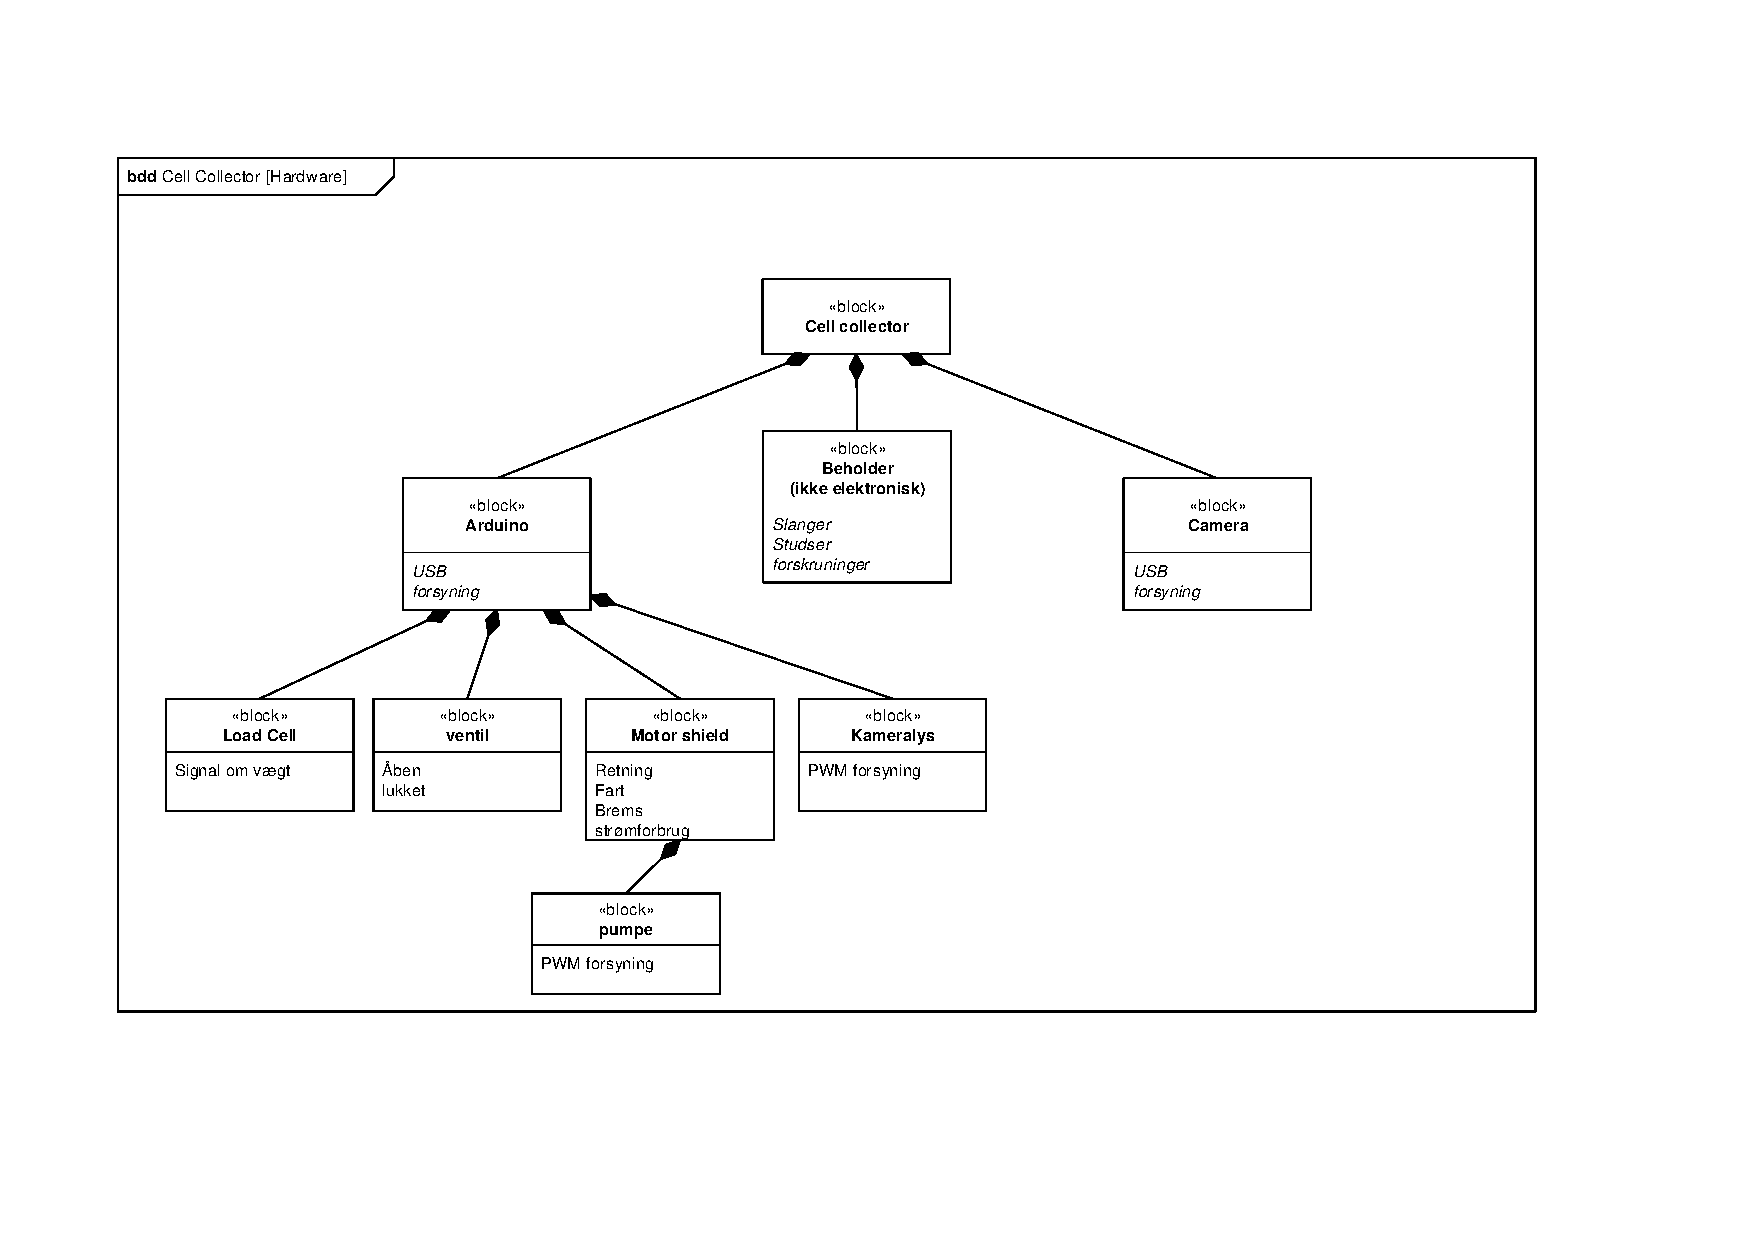
\includegraphics[width=1\textwidth]{pdf/BDD_Hardware.pdf}
	\caption{BDD - Cell Collector [Hardware]}
	\label{fig:bdd_Hardware}
\end{figure}
	
\newpage
\subsection{Internal block Diagram} 
Nedenstående IBD \ref{fig:ibd_Hardware} beskriver mere præcist, hvordan de forskellige komponenter interagerer med hinanden på. Diagrammet er brugt til, at der tidligt i udviklingsforløbet bliver defineret hvilke spændinger og signaltyper systemet skal indeholde. Systemet skal indeholde bestemte typer for, at kunne kommunikere med de interne dele.


\begin{figure}[H]
	\centering
	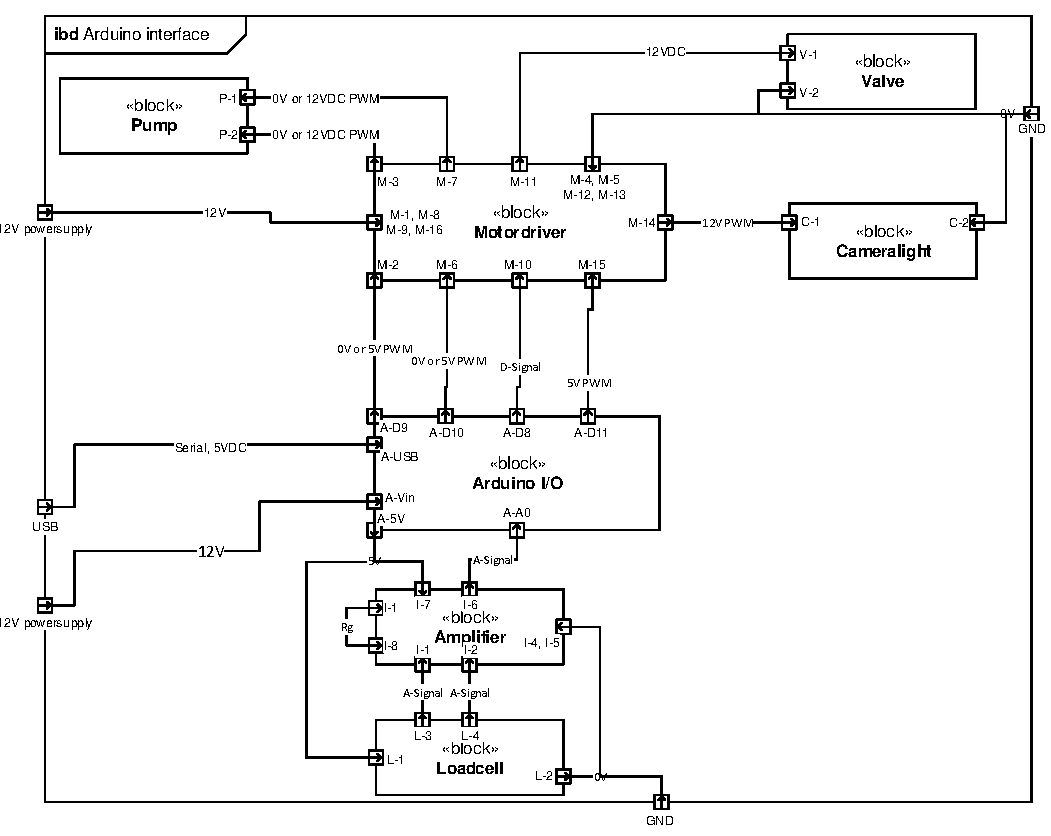
\includegraphics[width=1\textwidth]{pdf/IBD_Hardware(Arduino).pdf}
	\caption{IBD - Cell Collector [Hardware]}
	\label{fig:ibd_Hardware}
\end{figure}

\newpage
Tabellen nedenfor er brugt til at skabe en oversigt, over hvilke signaler og funktioner den enkle blok indeholder.

\begin{center}
		\begin{longtable}{ | m{2cm} | m{4.9cm}| m{3.45cm}| m{4.15cm}| } 
			\hline
			\textbf{Blok navn} &\textbf{Funktionsbeskrivelse} &\textbf{Signaler} &\textbf{Kommentar}\\ 
			\hline
			\multirow{2}{*}{Pump} & \multirow{2}{*}{Skabe flow i opløsningen} & 0V & Reference \\ 
& & 12VDC PWM & Strømforsyning \\	
			\hline	
			\multirow{2}{*}{Valve} & \multirow{2}{*}{Åbne og lukke for førringsveje} & 0V & Reference \\ 
& & 12VDC & Strømforsyning \\	
			\hline	
		\multirow{8}{*}{Motor shield} & \multirow{8}{*}{Forsyne ventil og pumpe} & 0V & Reference \\ 
& & 12V & Strømforsyning \\	
& & 0V or 5V PWM & Motor retning \\	
& & 0V or 5V PWM & Hastighedsregulering \\
& & Signal & Tænd/sluk ventil \\
& & 12V PWM & lysdiode lysintensitet \\
& & 0V or 12VDC PWM & Motor retning \\	
& & 0V or 12VDC PWM & Hastighedsregulering \\
			\hline	
			\multirow{5}{*}{Arduino} & \multirow{5}{*}{Styreenhed for hardware} & 0V & Reference \\ 
& & 12V & Strømforsyning \\	
& & USB & Seriel kommunikation og 5V \\
& & A-Signal & Aanalog indgangssignaler \\
& & D-Signal & Digital udgangssignaler \\
			\hline
			\multirow{3}{*}{Loadcell} & \multirow{3}{*}{Kontroller opløsningsbeholder} & 0V & Reference \\ 
& & 5V & Strømforsyning \\	
& & Signal & Udgangssignal \\	
			\hline
			\multirow{2}{*}{Cameralight} & \multirow{2}{*}{Lys til kameraet} & 0V & Reference \\ 
& & 12V PWM & Lysstyrke \\	
			\hline
		\end{longtable}
	\end{center}

	
\newpage
Tabellen nedenfor beskriver signalerne der findes i systemet, denne tabel anvendes når grænsefladerne skal designes og testes.

\begin{center}
		\begin{longtable}{ | m{2cm} | m{5.5cm}| m{2cm}| m{1.250cm}| m{1.250cm}| m{2.5cm}| } 
			\hline
			\textbf{Signal navn} &\textbf{Funktionsbeskrivelse} &\textbf{Område} & \textbf{Output} & \textbf{Input} &\textbf{Kommentar}\\ 
			\hline
			\multirow{2}{*}{0V} &  \multirow{2}{*}{Reference til analoge  spændinger} & N/A & GND & V-2  & Stel \\ 
& & & GND & C-2 &   \\
& & & GND & I-4, I-5 &   \\
& & & GND & M-4, M-5, M-12, M-13 &   \\
			\hline	
			USB &  Seriel kommunikation & & USB & A-USB &  \\ 
			\hline	
			5V & \multirow{2}{*}{Forsyningsspænding} & 4.9-5.1V & A-5V & I-7 & 5V fra USB  \\ 
& & & A-5V & L-1 & \\
			\hline
			12V & \multirow{2}{*}{Strømforsyningsspænding} & 11.9-12.1V & 12V PS & A-Vin & \\
			& & & 12V PS & M-1, M-8, M-9, M16 &   \\ 
			\hline
			PWM & Forsyningsspænding & 0V eller 5V & &  & Digital \\ 
			\hline	
			A-Signal(mV) &\multirow{2}{*}{Registrering af fysiske værdier}  & 0-5mV & L-3 & I1 & Analog fra vægtcelle \\ 
			& & & L-4 & I-2 &  Analog fra vægtcelle \\
			\hline
			A-Signal(V) & Registrering af fysiske værdier & 0-5mV & I-6 & A-A0 & Analog fra amplifier\\ 
			\hline
			D-Signal() & Styring af ventil & 4.9-5.1V & A-D8 &M-10 & \\ 
			\hline
			0V or 12V PWM & \multirow{2}{*}{Forsyning til pumpe} & 0 eller 12V & M-3 & P-2 & \\
			& & & M-7 & P-1 & \\
			\hline	
			12VDC & Forsyning til ventil & 11.9-12.1V & M-11 & V-1 &  \\
			\hline
			12V PWM & Forsyning til lysdioder & 4.9-5.1V & A-D11 & M-15 &  \\
			\hline
			5V PWM & Styring af lysdioder & 4.9-5.1V & A-D11 & M-15 &  \\
			\hline
			0V or 5V PWM & \multirow{2}{*}{Styring af pumpe} & 0 eller 12V & A-D9 & M-2 & Hastighed og retning\\
			& & & A-D10 & M-6 & \\
			\hline
		\end{longtable}
	\end{center}


\newpage
\subsection{Kamera}
\label{subsec:Kamera}
Kameraet[\citet{DH2}] skal detektere de langerhanske øer i systemet, hvilket gør at det er en elementær del af projektet.

\textbf{Specifikationer for kameraet:} 
\begin{center}
		\begin{longtable}{ | m{6.5cm} | m{6.5cm}| } 
			\hline
			\textbf{Specifikation} &\textbf{Værdi} \\ 
			\hline
			\textbf{Billede opløsning:} & 2M pixel \\ 
			\hline
			\textbf{Fokus område:} & 0-40mm  \\ 
			\hline
			\textbf{forstørrelse:} & 25X-400X (Manuelt)  \\ 
			\hline
			\textbf{Frame rate:} & 30f/s  \\ 
			\hline
			\textbf{Interface:} & USB 2.0  \\ 
			\hline
			\textbf{Forsyning:} & DC 5V (\textit{fra USB port})  \\ 
			\hline
			\textbf{Dimension:} & L:\SI{112}{\milli\metre} x B:\SI{33}{\milli\metre}  \\ 
			\hline			
		\end{longtable}
		
	\end{center}
Da Langerhanske øer har en størrelse på \SI{100}{\micro\metre} til \SI{300}{\micro\metre}, skal kameraet have en opløsning så øerne kan detekteres. Opløsningen på kameraet er valg ud fra:
\begin{align}
\text{Opløsning} = \frac{\text{Afstand}}{\text{Objektstørrelse}} = \frac{\SI{10}{\centi\metre}}{\SI{100}{\micro\metre}} 
\end{align} \citep[s.5]{DH1}
afstanden fra objektet er vurderet ud fra, hvor langt kameraet er i den absolut maksimale afstand fra øerne. Dertil skal der kunne ses flere detaljer end ned til \SI{100}{\micro\metre}, for at kunne detektere de langerhanske øer. Derfor er der valgt et kamera med en opløsning på 2M pixels. Da de Langerhanske øer er lysere og har et andet fluorescens niveau end resten af vævet vil et kamera uden farver også være anvendeligt. Da systemet skal kunne sortere 30 langerhanske øer i minuttet, er det vurderet at en standard frame rate vil være passende. Til projektet er der taget et valg mellem 3 kamera, det valgte er listet oven over og de 2 fra valgte er i tabellen her under.

\begin{center}
		\begin{longtable}{ | m{3cm} | m{9.5cm}| } 
			\hline
			\textbf{Kamera type} & USB Microscope Digital-Mikroskop Endoskop[\citet{DH9}] \\ 		
			\hline
			\textbf{Billede opløsning} & 2M pixel \\ 
			\hline
			\textbf{Fokus område:} & n/a  \\ 
			\hline
			\textbf{forstørrelse:} & 50X-800X (Manuelt)  \\ 
			\hline 
			\textbf{Frame rate:} & n/a  \\ 
			\hline
			\textbf{Interface:} & USB (ukendt version)  \\ 
			\hline
			\textbf{Forsyning:} & DC 5V (\textit{fra USB port})  \\ 
			\hline
			\textbf{Dimension:} & L:\SI{112}{\milli\metre} x B:\SI{33}{\milli\metre}  \\ 
			\hline	
			\textbf{Pris:} & 148,33kr.\\ 
			\hline
		\end{longtable}
	\end{center}
	
	\begin{center}
		\begin{longtable}{ | m{3cm} | m{9.5cm}| } 
			\hline
			\textbf{Kamera type} & AVEN ZIPSCOPE[\citet{DH10}] \\ 		
			\hline
			\textbf{Billede opløsning} & 2M pixel \\ 
			\hline
			\textbf{Fokus område:} &  10mm-500mm (Manuelt) \\ 
			\hline
			\textbf{forstørrelse:} & 10x-50x (Optisk), 200X (Digital)  \\ 
			\hline
			\textbf{Frame rate:} & 30f/s  \\ 
			\hline
			\textbf{Interface:} & USB 2  \\ 
			\hline
			\textbf{Forsyning:} & DC 5V (\textit{fra USB port})  \\ 
			\hline
			\textbf{Dimension:} & n/a \\ 
			\hline	
			\textbf{Pris:} & 1734,15kr.\\ 
			\hline
		\end{longtable}
	\end{center}
	
Prisen for det indkøbte Kamera var 264,15kr., hvilket har været på et middel prisniveau ud fra de tre kamera. Grunden til valget af det Indkøbte præger af prioritering af et ordenligt datablad og et stramt budget.

%Kameraet skal detektere de langerhanske øer, når de kommer forbi i slangen.  Da de langerhanske øer skiller sig ud ved at være mere lyse end resten af vævet, vil det være underordnet om kameraet er et farve kamera. Da systemet ikke skal operere under en stor hastighed er en standard frame rate valgt på 30 f/s. Kameraet opløsningen er valgt ud fra, at det skal kunne se de langerhanske øer med en størrelse på 100-300um. Til bestemmelse til dette er der brugt følgende formel:
 %\fixme{Mangler formel}
%For at kameraet har mulighed for, at se lidt flere detaljer og forhåbning om at det kan være tættere på end 10 cm, er det besluttet er et 2 megapixels kamera burde være passende.


 
\newpage
\subsection{Styreenheden}
Microcontrolleren skal være styrerenheden i systemet, det betyder at den skal styre ventil, kameralyset, pumpe og vægtcelle.  

\textbf{Specifikationer for Microcontroller[\citet{DH3}]:} 
\begin{center}
		\begin{longtable}{ | m{6.5cm} | m{6.5cm}| } 
			\hline
			\textbf{Specifikation} &\textbf{Værdi} \\ 
			\hline
			\textbf{Type:} & Arduino UNO (ATmega328P) \\ 
			\hline
			\textbf{Forsyning:} & 5VDC (USB)  \\ 
			\hline
			\textbf{Clock speed:} & 16 MHz  \\ 
			\hline		
			\textbf{Digitale I/O pins:} & 14 stk (6 stk med PWM)  \\ 
			\hline	
			\textbf{Analoge inputs pins:} & 6 stk  \\ 
			\hline	
			\textbf{Interface:} & USB  \\ 
			\hline	
			\textbf{I/O output strøm:} & 20 mA  \\ 
			\hline
			\textbf{Flash hukommelse:} & 32 KB  \\ 
			\hline	
		\end{longtable}
\end{center}
Arduino er en open source platform til fremstilling af prototype print, med en ATmega328P microcontroller. Arduino platformen er valgt da Matlab understøtter interaktion via en Support package. Boardet er brugt i et stort omfang omkring i verden. Derfor er det en platform der er nemt tilgængelig og forholdsvis prisvenlig, samt at der findes en stor mængde dokumentation omkring emnet. Da det er en open source platform, kan der købes forskellige versioner som ikke er originaler. Arduino UNO er passende til dette system, da det er en forholdsvis simpel opgave microcontrolleren skal håndtere. Da systemet bruger computerens hukommelse og det meste er koden her på. Antallet af digitale og analoge porte er passende med den nuværende mængde af komponenter der skal styres. 

\subsection{Motordriver}
Motordriveren skal hjælpe microcontrolleren med, at styre pumpen og ventilen til systemet. Det skal den fordi Arduinoen ikke kan trække pumpen alene, derfor skal der en ekstern forsyningskilde på, som forsynes i gennem motor shieldet. Motordriveren skal også forsyne ventilen. 

 \textbf{Specifikationer for Motordriver[bilag \ref{bilag:L293D}]:} 
\begin{center}
		\begin{longtable}{ | m{6.5cm} | m{6.5cm}| } 
			\hline
			\textbf{Specifikation} &\textbf{Værdi} \\ 
			\hline
			\textbf{Type:} & L293D \\ 
			\hline
			\textbf{Forsyning:} &  4,5-36V \\ 
			\hline
			\textbf{Output spænding} & 4,5-36V  \\ 
			\hline		
			\textbf{Output strøm} & 600mA per kanel  \\ 
			\hline	
			\textbf{Kanaler} & 4 stk  \\ 
			\hline	
			\textbf{Interface} & Strømforsyning og arduino  \\ 
			\hline	
		\end{longtable}
\end{center}
Motordriveren kan levere 600mA pr. kanal hvilket er nok til at forsyne pumpe og ventil. Derudover køres der PWM til den som gives videre til pumpe og ventil. Motordriveren har desuden også den fordel, at den er galvanisk adskilt fra Arduinoen. og derved ikke kan nedlægge Arduinoen mm. Ydermere giver den også mulighed for at overvåge strømforbruget på dens kanaler. Det kan være med til at beskytte pumpens motor.


\subsection{Ventil} \label{design_ventil}
Ventilens funktion er at sortere de langerhanske øer, fra resten af opløsningen. Det gør den ved at Arduinoen giver den besked om, at åbne og lukke for ventilen.

\textbf{Specifikationer for Ventil[bilag \ref{bilag:161T031}]:} 
\begin{center}
		\begin{longtable}{ | m{6.5cm} | m{6.5cm}| } 
			\hline
			\textbf{Specifikation} &\textbf{Værdi} \\ 
			\hline
			\textbf{Type:} & Solenoid Electromagnet Valve \\ 
			\hline
			\textbf{Forsyning:} & 12VDC, 0.1A  \\ 
			\hline
			\textbf{Porte} & 3 stk \\ 
			\hline		
			\textbf{studser} & 1mm  \\ 
			\hline	
			\textbf{Åbningstid} & <20ms  \\ 
			\hline	
			\textbf{Lukningstid} & <30ms  \\ 
			\hline	
			\textbf{Interface} & open/closed  \\ 
			\hline	
		\end{longtable}
\end{center}
Ventilen er en vigtig del af systemets hardware, da det er dens ansvar at sortere de detekterede øer fra resten af væsken. Det er svært at finde ventiler med \SI{500}{\micro\metre} studser. Det kan godt lade sig gøre at få adaptere så større ventiler kan bruges, men sporbarheden omkring hvor den enkelte ø befinder sig, forsvinder hvis kammeret pludseligt bliver stort. Der er utrolig stor variation i kvalitet og pris på magnetventiler. Ventilen er et hardware, hvor der kan bruges meget tid og mange penge i projektet.
Kravene til ventilen er, at den skal være 3 vejs med 1 tilgang og 2 udgange, yderligere skal studserne kunne tilpasses slange størrelsen, være til væske og have en lukke/åbne tid under 50 ms.
For at kunne bruge ventilen er det vigtigt at forstå ventilens opbygning. 
 En magnetventil virker på den måde at den består af en spole, der danner et magnetfelt når der bliver påsat spænding og derved trækker et stempel til sig. Det får ventilen til at åbne ved hjælp af en membran. En trevejs magnetventil, som den brugte i dette projekt virker på samme måde. Men hvor skifter position er designet så der altid er en åben. Derfor vil opløsningen løbe ud i wastebeholderen når der ikke er en langerhanske ø, men kommer der en vil den skifte position, hvorved de bliver frasorteret. Se figur \ref{fig:ventilpos} for en illustration af en 3 vejs magnetventil.

\begin{figure}[H]
	\centering
	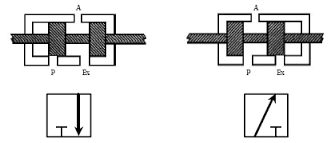
\includegraphics[width=0.5\textwidth]{billeder/Hardware/ventil.png}
	\caption{Magnetventil position}
	\label{fig:ventilpos}
\end{figure}  

For at sorteringen af langerhanske øer er succesfuld, kræver det en beregning af hastigheden det tager for en langerhansk ø, at komme fra kameraet til ventilen.En estimation er beregnet igennem nedenstående formler. Kravet fra kunden hedder 30 øer i minuttet, derfor skal systemet som minimum have en flow hastighed på 11,25 ml/min. Se formel \ref{eg:ohastighed} for udregningen. På figur \ref{fig:tidsintervalventil} kan der ses en illustration af problemstillingen 

\begin{figure}[H]
	\centering
	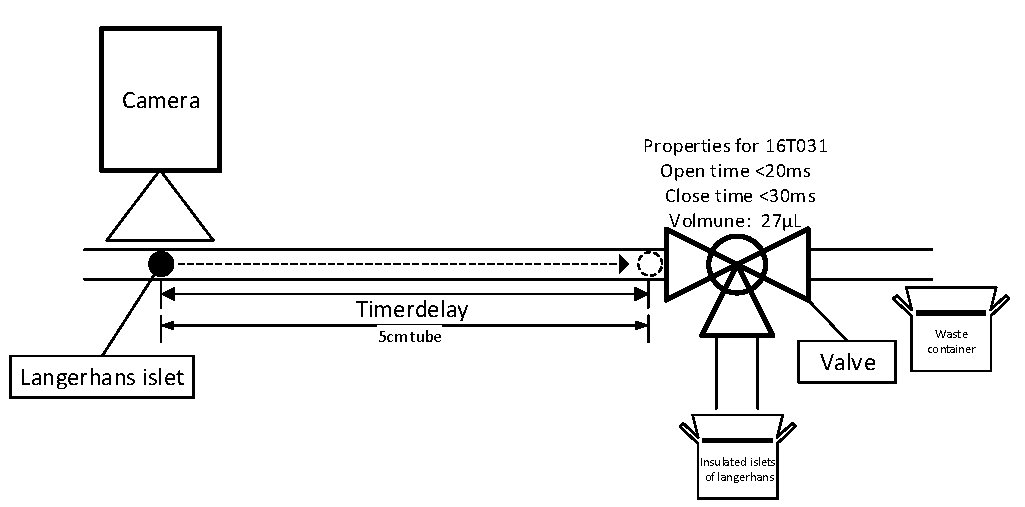
\includegraphics[width=1\textwidth]{billeder/tidsinterval.pdf}
	\caption{Illustration af ventil timerdelayet}
	\label{fig:tidsintervalventil}
\end{figure}

\begin{align}
\frac{\text{Opløsningsstørrelse}}{\text{Antal øer i opløsning}} = \frac{\SI{150}{\milli\liter}}{400\text{ øer}}*30\text{ øer/minut} = \SI{11,25}{\milli\liter/minut} 
\label{eg:ohastighed}
\end{align}(\textit{jf. Søren Gregersen})

Tiden i mellem kameraet og ventilen kan estimeres ud fra det volumenet af slangen, i i mellem de to komponenter \ref{eg:slangevolume}.

\begin{align}
V=\pi*r^2*h=\pi*(\frac{\SI{0,51}{\milli\metre}}{2})^2*\SI{50}{\milli\metre}=\SI{0,010214}{\milli\liter}
\label{eg:slangevolume}
\end{align}

Det vil sige at med et flow på $\SI{11,25}{\milli\liter/minut}$, som er beregnet ud fra formlen \ref{eg:ohastighed} kan tiden fra kamera til ventil beregnes ved formel \ref{eq:tidsintervallet}. 
 
\begin{align}
\frac{\SI{0,010214}{\milli\liter}}{\frac{\SI{11,25}{\milli\liter/minut}}{\SI{60}{\second}}}\to\frac{\SI{0,010214}{\milli\liter}}{\SI{0,1875}{\milli\liter/s}}=\SI{0.054475}{\second}
\label{eq:tidsintervallet}
\end{align} 

I følge bilag \ref{bilag:ventil} har ventilen et volumen på $\SI{27}{\micro\liter}$. Til at beregne tiden det tager, at tømme ventilen bruges formel \ref{eq:ventilvolume}. %\label{eq:ventilvolume}.

\begin{align}
\text{Tid for udtømning af ventilen} = \frac{\text{ventil volume}}{\text{ml pr. sekund}}=\frac{\SI{27}{\micro\liter}}{\SI{0,1875}{\milli\liter/s}}=\SI{144}{\milli\second}
\label{eq:ventilvolume}
\end{align}

Beregninger til ventilen skal bruges i softwaren til at implementere timere til styring af ventilen. Åbnings- og lukningstid skal beregnes med i tiden til disse, se afsnit \ref{software_ventil} for implementeringen af timerne og yderligere udregninger.

\newpage
 På figur \ref{fig:ventildiagram} kan der ses et diagram over arduinoen, motordriveren, ventilen og en diode som indikator for at ventilen er åben. Ligesom ved motoren er det også her nødvendigt, at sætte en modstand foran lysdioden. Modstanden er af samme type som til kameralyset se \ref{subsec:kameralys} for beregninger for dem.

\begin{figure}[H]
	\centering
	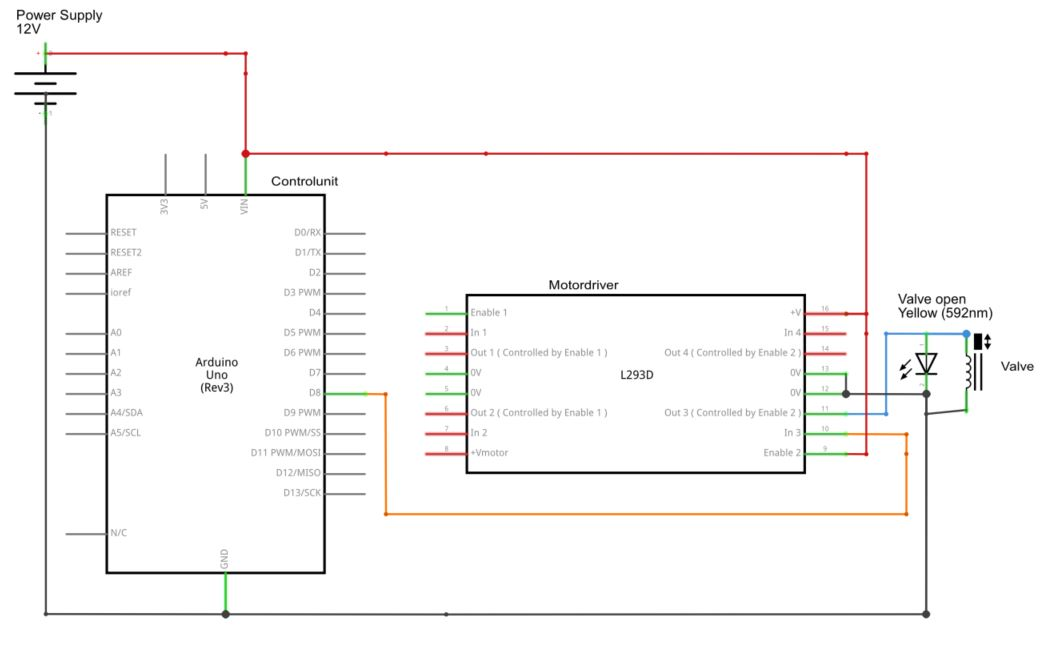
\includegraphics[width=1\textwidth]{billeder/Hardware/diagrammer/ventildiagram.JPG}
	\caption{Kredsløbsdiagram for ventil}
	\label{fig:ventildiagram}
\end{figure} 

\newpage
\subsection{Pumpe}
Pumpen skal skabe det nødvendige flow i væsken fra det ene punkt til det andet. Flowet skal være lavt nok til at kameraet kan nå at detekterer en ø.

\textbf{Specifikationer for Pumpe[\citet{DH8}]:} 
\begin{center}
		\begin{longtable}{ | m{6.5cm} | m{6.5cm}| } 
			\hline
			\textbf{Specifikation} &\textbf{Værdi} \\ 
			\hline
			\textbf{Type:} & Peristaltisk pumpe \\ 
			\hline
			\textbf{Forsyning:} & 12VDC, 0,3A  \\ 
			\hline
			\textbf{Hastighed} & (2-17mL/min) \\ 
			\hline		
			\textbf{studser} & ID:1mm OD:3,3mm  \\ 
			\hline	
		\end{longtable}
\end{center}

Det er et krav at pumpens flow hastighed er variabel, så flowet kan justeres. Der findes mange forskellige pumpetyper til formålet, herunder stempel pumper, peristaltiske pumper og vakuum pumper. Der er bestilt en peristaltisk pumpe som virker ved at klemme på slangen og derved skabe et flow, det skal dog undersøges hvordan de langerhanske øer vil opfører sig ved sådan en pumpe. Undersøgelserne bør bestå af om de langerhanske øer tager skade ved, at pumpen klemmer på slangen.

\subsubsection{Motordriver}
Til at drive pumpen er det nødvendigt med en motordriver, fordi arduinoen langt fra kan leverer den nødvendige strøm til pumpen. Kravet til motordriveren er, at den kan trække pumpen, samt stadig have mulighed for regulering af pumpens hastighed.
Motordriveren består i dette projekt af en L293D, som enten kan drive 4 motorer den ene vej, 2 motorer i begge retninger eller i dette tilfælde en Peristaltisk pumpe, en magnetventil og kameralyset. se figur \ref{fig:L293DInterndiagram} for L293D interne kredsløb diagram. 
 
   \begin{figure}[H]
	\centering
	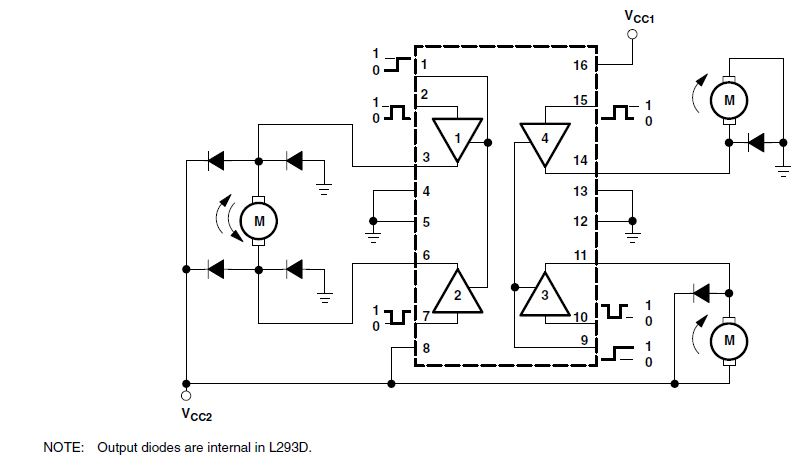
\includegraphics[width=0.9\textwidth]{billeder/Hardware/diagrammer/L293intern.JPG}
	\caption{Intern kredsløbsdiagram for L293D}
	\label{fig:L293DInterndiagram}
\end{figure}

Motordriverens opgaver er forsyne motoren, i sin simple form skal L293D tage signalet fra arduinoen, analysere det og give et tilsvarende signal fra strømforsyning til motoren.
\subsubsection{Hastighedscontrol af pumpe}
Da det er svært at finde en pumpe der præcis opfylder kravet til hastigheden i dette system, grundet de 30 øer i minuttet(\ref{subsec:Kvalitetskrav}.1)
\begin{align}
\frac{\text{Opløsningsstørrelse}}{\text{Antal øer i opløsning}} = \frac{150}{400}*30 = 11,25ml/min
\label{eg:ohastighed}
\end{align}(\textit{jf. Søren Gregersen})
Der er 3 primært metoder til, at styre hastigheden på en DC-motor \citep{ELengbog}s.810.

1. Indsætte modstand i kredsløbet før motoren er koblet til.
Denne metode kan bruge på alle typer af motorer. En simpel måde er at gøre det på er, at sætte en variabel modstand i serie med motoren for, at styre hastigheden. Ulemperne ved dette kredsløb er at ,forbruget vil være ens ved den højeste hastighed og den laveste. Det vil det fordi modstanden vil blot omsætte energien til varme, hvilket vil være spild af energi. Se figur \ref{fig:motormodstand}, princippet er baseret på KVL.

\begin{figure}[H]
	\centering
	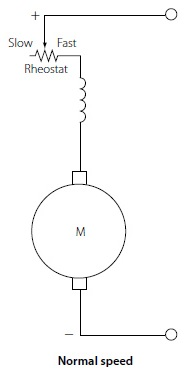
\includegraphics[width=0.3\textwidth]{billeder/Hardware/motormodstand.jpg}
	\caption{Kredsløbsdiagram for Motor med variablemodstand}
	\label{fig:motormodstand}
\end{figure}

2. Variere strømmen der tilføres motoren, hvor spændingen holdes konstant.
Denne metode minder om den overstående, men i stedet for serie kobles den variable modstand parallelt, som det kan ses på figur \ref{fig:motorcurrent}. Ulempen ved dette kredsløbt er at når motoren skal køre ved lav hastighed, er modstanden lille og derved tæt på en kortslutning derfor er det vigtigt, at kredsløbet er designet rigtigt. Princippet er baseret på KCL.

\begin{figure}[H]
	\centering
	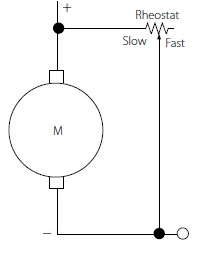
\includegraphics[width=0.3\textwidth]{billeder/Hardware/motorcurrent.jpg}
	\caption{Kredsløbsdiagram for Motor med variable strøm}
	\label{fig:motorcurrent}
\end{figure}

\fxnote{hvis tiden er til det, kan der uddybes med generel motor teori som opbygning mm. Derud over kunne der sagtens lave nogle formler også til generelle motorer, så som moment mm.}


3. Variere spændingen der tilføres motoren periodevis, hvor strømmen holdes konstant.
Konceptet i denne metode er at have en konstant forsyning, som slukkes og tændes for, sagt på en simpel måde. Dvs. at der sidder en kontakt i mellem strømforsyningen og motoren, der tændes og slukkes. Kredsløbet for dette kan stilles op som figur \ref{fig:motorkontakt} og giver et signal som på figur \ref{fig:onoffwave}

 \begin{figure}[htbp] \centering
\begin{minipage}[b]{0.48\textwidth} \centering
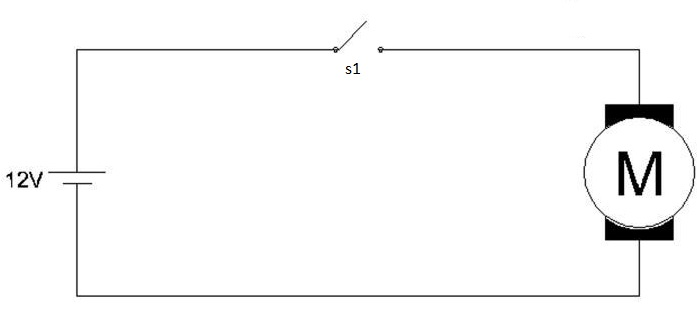
\includegraphics[width=1.00\textwidth]{billeder/Hardware/motorkontakt.jpg} % Left picture
\end{minipage} \hfill
\begin{minipage}[b]{0.48\textwidth} \centering
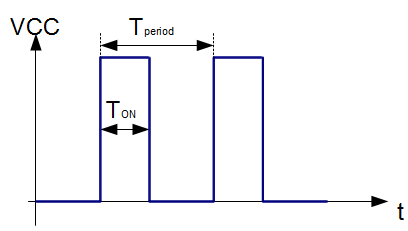
\includegraphics[width=1.00\textwidth]{billeder/Hardware/onoffwave.jpg} % Right picture
\end{minipage} \\ % Captions og labels
\begin{minipage}[t]{0.48\textwidth}
\caption{Kredsløbsdiagram for Motor med en kontakt} % Left caption and label
\label{fig:motorkontakt}
\end{minipage} \hfill
\begin{minipage}[t]{0.48\textwidth}
\caption{Motorsignal ved periodevis spænding } % Right caption and label
\label{fig:onoffwave}
\end{minipage}
\end{figure}
Åbningstiden $T_{on}$ er der hvor kontakten er tændt, $T_{period}$ er perioden som kontakten åbner og lukker. Den gennemsnitlige spænding kan regnes ud ved \ref{eq:VT}

\begin{align}
V_T=V_S \frac{T_{on}}{T_{period}}
\label{eq:VT}
\end{align}
Ud fra overstående formel (\ref{eq:VT}) ses det, at gennemsnit spændingen og derved også hastigheden på motoren styres ved $T_{on}$ altså hvor langtid kontakten er tændt. Denne form for styring af en motor, kaldes også pulse width modulation.



\paragraph{Pulse width modulation} \phantom{mmmmmmmmmmmmmmmmmkkkkkkkkkkkkkkkkkkkkkkkkkkkkkkkkmmmmmmmmmmmmmmmmmmmmmm}

Pulse width modulation(PWM) er en meget brugt metode som kan bruges til, at styre hastigheden på en DC motor. Dette gøres ved at tænde og slukke for en digital udgang. Det er duty cyklussen der får hastigheden til at varierer, dvs. at det er tiden hvor det firkantede signal er "højt" der bestemmer hastigheden. Da strømforsyningen er 12V og motoren kun kan tåle 6V, betyder det at duty cyklussen ikke må overstige 50\%, da det vil give en højere gennemsnits spænding end 6V, hvilket er motorens maksimale spænding. Se figur \ref{fig:pwmsignal} for illustration af PWM duty cyklusser og gennemsnit spændinger. PWM styring kan bruges til blandt andet dæmning af dioder, generering af lydsignaler og styring af motorer \fxnote{højere fagligt sprog og niveau og nogle gode referencer}. 

 \begin{figure}[H]
	\centering
	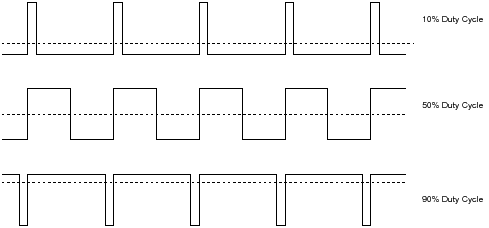
\includegraphics[width=0.8\textwidth]{billeder/Hardware/pwm.png}
	\caption{PWM duty cyklusser med gennemsnits spændinger}
	\label{fig:pwmsignal}
\end{figure}

Der er flere metoder, hvor dette kan implementeres vha. arduinoen. Den mest simple metode er $analogWrite(pin, dutyCycle);$ hvor dutycycle er en værdi mellem 0 og 255 og pin er en af de digital udgange med PWM. Dette er simpelt, men der er ingen control over frekvens mm. 

Manuel PWM implementering er en anden metode, der kan implementeres således:

\begin{lstlisting}
void setup()
{
  pinMode(13, OUTPUT);
}

void loop()
{
  digitalWrite(13, HIGH);
  delayMicroseconds(100); // Approximately 10% duty cycle @ 1KHz
  digitalWrite(13, LOW);
  delayMicroseconds(1000 - 100);
}
\end{lstlisting}

Her sættes pin 13 til \textit{høj}, hvor efter der ventes 100 mikro sekunder. Derefter sættes pin 13 \textit{lav} og der ventes 900 mikro sekunder. Ved denne metode kan alle digitale udgange bruges og ikke kun dem med PWM. Dog er processeren brugt hele tiden da den også bruges når der ventes. Det vil sige at den ikke kan bruges til andet samtidigt, hvilket ikke kan bruges i projektet.
Microcontrolleren der sidder på arduinoen indeholder 3 timere, som kan bruges til PWM generering.  Måden dette virker på er at timeren går fra 0 til 255, hvis $Timer=0$ sættes outputtet højt, hvor den tæller til enten 255 og slukker hvilket vil skabe en duty cyklus på 100\%. Derfor kan der defineres en værdi hvor der slukkes mellem 0 og 255. Ydermere findes der scalar (1, 8, 64, 256 eller 1024 som divideres med arduinoens clock frekvens. Alt dette konfigureres ved bits i registre (TCCRnA og TCCRnB) på microcontrolleren. Et eksempel på dette kunne være: 

\begin{lstlisting}
void setup()
{
pinMode(3, OUTPUT);
  pinMode(11, OUTPUT);
  TCCR2A = _BV(COM2A1) | _BV(COM2B1) | _BV(WGM21) | _BV(WGM20);
  TCCR2B = _BV(CS22);
  OCR2A = 180;
  OCR2B = 50;
\end{lstlisting}

Ved overstående kode vil der være en duty cyklus på output A da være $$\frac{180+1}{256}*100=70,7\%$$ og en PWM frekvens på     
  $$\frac{16MHz}{64/256}=976.6Hz$$. Output B vil have en duty cyklus på $$\frac{50+1}{256}*100=19.9 \%$$ og den samme frekvens. Den sidst nævnte metode, er den metode hvor der er mest kontrol over PWM signalet. Derfor bruges denne i dette projekt.
  
For at lysdioderne får deres ønskede spænding, er det nødvendigt med modstande foran dem. Modstandene kan beregnes på følgende måde. 
\begin{align}
R=\frac{V_{source}-V_{lysdiode}}{I_{lysdiode}}=\frac{6-3.2}{20mA}=140\Omega
\label{eq:modstandLEDmotor}
\end{align} 
Dette giver en effekt afsætning i modstandene på $(V_{source}-V_{lysdiode}*I_{lysdiode}=2,8*20mA=0,056W)$ hvilket giver grund for at 0.33W modstande er passende.

% Der er også købt en vakuum pumpe, som muligvis kan sidde efter ventilen. Der skal dog stadig skabes et flow til de sorterede øers beholder, måske en kombination vil være det optimale. En modultest af de enkelte pumper skal afgøre hvilken løsning der er den mest optimale. 
På figur \ref{fig:motordriverdiagram} kan ledningsdiagrammet til motordriver med motor og frem og tilbage lysdioder observeres. Med opsætningen kan retningen på motoren bestemmes ved, hvilken en af udgangene der sættes til lav(0V). Hvor den modsatte udgang konfigureres til PWM. Gøres det modsat kører motoren den modsatte vej.
 
 \begin{figure}[H]
	\centering
	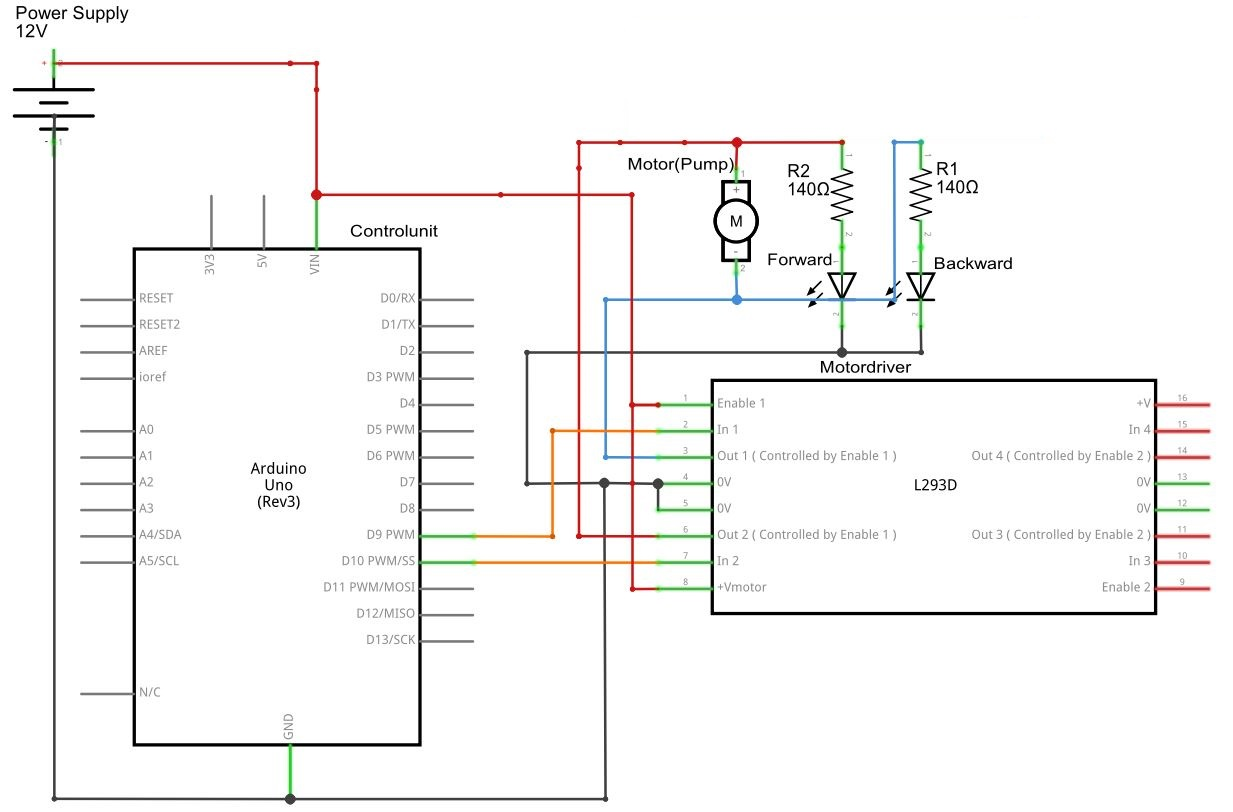
\includegraphics[width=1\textwidth]{billeder/Hardware/diagrammer/motordiagram.JPG}
	\caption{Kredsløbsdiagram for motor og motordriver}
	\label{fig:motordriverdiagram}
\end{figure}


\subsection{Vægtcelle}
\label{subsec:loadcell}
Vægtcellen skal bruges til at kontrollere om, der er væske i celleopløsningsbeholderen.

\textbf{Specifikationer for Vægtcelle[\citet{DH7}]:} 
\begin{center}
		\begin{longtable}{ | m{6.5cm} | m{6.5cm}| } 
			\hline
			\textbf{Specifikation} &\textbf{Værdi} \\ 
			\hline
			\textbf{Max belastning:} & 1 kg \\ 
			\hline
			\textbf{Anbefalet arbejdsspænding} & 3-12V \\ 
			\hline
			\textbf{Output} & 1.0mV/V$\pm$0.15mV/V \\ 
			\hline
		\end{longtable}
\end{center}

Den indkøbte vægtcellen kan veje op til 1 kg, hvilket fint dækker vægten for celleopløsningsbeholderen på 250ml + beholderens vægt.

 For at kunne udnytte funktionen af en vægtcelle, skal opbygningen af denne forstås. En vægtcelle måler hvor meget vægt den udsættes for vægtcellen, der er brugt i projektet, består af strain gages koblet i en wheatstone bro. En strain gage bruges til at måle fysisk stræk eller kompression. Den er simpel i sin opbygning ved at består af en meget tynd elektrisk ledende tråd, som er ført frem og tilbage på et elastisk folie, hvilket er illustreret på \ref{fig:Strain gages}\footnote{kilde: \url{https://en.wikipedia.org/wiki/Strain_gauge}}. 
 
 \begin{figure}[H]
	\centering
	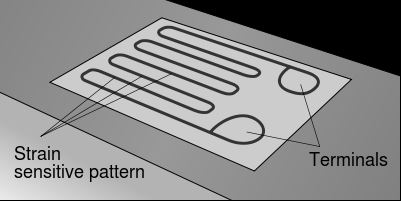
\includegraphics[width=0.5\textwidth]{billeder/Hardware/straingages1.JPG}
	\caption{illustration af strain gages}
	\label{fig:Strain gages}
\end{figure}

En strain gages modstand stiger ved stræk og falder ved kompression, dette kan beskrives ud fra formlen \ref{eq:modstandsformel}\citep{Websterbog}{s.47}

 \begin{align}
 R=\frac{\rho*L}{A}
 \label{eq:modstandsformel}
 \end{align}
 
 Hvor R=modstand, $\rho$=modstand per meter, L=længden og A=tværsnitsarealet. Der er mere til formlen en dette, bla. materiales egenskaber og temperatur. På vægtcellen er der fire strain gages, som er placeret på vægtcellen på denne måde som vist på figur \ref{fig:Loadcell1}. Strain gages R1 og R4 bliver strukket, hvor R2 og R3 på undersiden bliver skubbet sammen.
 
 Måden de er forbundet er vist på figur \ref{fig:loadcell2}, denne metode at koble modstande på kaldes en wheatstone bro\citep{ELengbog}{s.122}. mere specifikt for denne er også kendt som et full-bridge kredsløb\citep{AETbog}{s.76}. Forholdet mellem input spændingen og output spændingen kan beskrives, som vist ved formlen\ref{eq:fullbformel}
\begin{align}
 V_{out}=GF*V_{in}*\varepsilon
 \label{eq:fullbformel}
 \end{align}
 Hvor V$_{out}$=udgangssignalet, V$_{in}$=indgangsspændingen , GF=gages factor som er materialets egenskab og $\varepsilon$=strukket der er tilført til vægtcellen.

\begin{figure}[htbp] \centering
\begin{minipage}[b]{0.48\textwidth} \centering
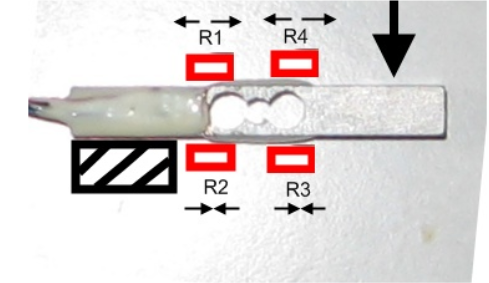
\includegraphics[width=1.00\textwidth]{billeder/Hardware/loadcell1.PNG} % Left picture
\end{minipage} \hfill
\begin{minipage}[b]{0.48\textwidth} \centering
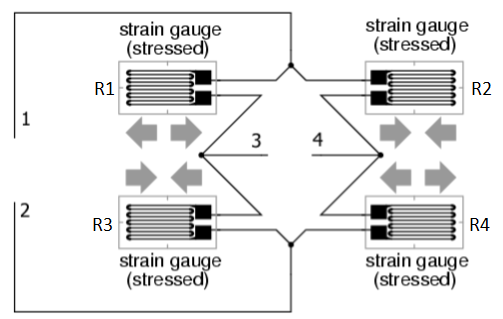
\includegraphics[width=1.00\textwidth]{billeder/Hardware/straingages2.PNG} % Right picture
\end{minipage} \\ % Captions og labels
\begin{minipage}[t]{0.48\textwidth}
\caption{Illustration af strain gages i loadcell på virkning} % Left caption and label
\label{fig:Loadcell1}
\end{minipage} \hfill
\begin{minipage}[t]{0.48\textwidth}
\caption{Illustration af koblingen strain gages i loadcell} % Right caption and label
\label{fig:loadcell2}
\end{minipage}
\end{figure}

Ud fra databladet \ref{subsec:loadcell} ses det, at output spændingen er 1.0mV pr volt på indgangsspændingen. Dette er pga. det meget lille strain der tilføres til emnet, hvilket også er med til at strain gagesene ikke går i stykker. Da Arduinoens analog til digital konverter er 10bit, hvilket vil sige $2^{10}=1024$ det betyder at konverteren har 1024 trin fra 0 til 1023. Konverterens arbejdsspænding går fra 0 V til 5 V. 

\begin{align}
 \text{Spænding per trin}=\frac{\text{Maksimale spænding}}{\text{Antal trin}}=\frac{5 V}{1024\text{ trin}}=0,0049V=4,9mV
 \label{eq:volt-step}
 \end{align}
 
I \ref{eq:volt-step} viser det sig at den mindste værdi ADC kan måle er 4,9mV, dette medfører at arduinoen maksimalt vil måle et step ved 1kg på vægtcellen, da $1mV*5V=5mV$. Dette giver to valgmuligheder
\begin{enumerate}
\item Anskaffe en bedre ADC, bestående af flere bits
\item Hæve udgangsspændingen fra vægtcellen 
\end{enumerate}
I dette tilfælde vælges punkt 2, at hæve udgangsspændingen fra vægtcellen. 
\subsubsection{Forstærkning af signal}
Til dette formål bruges en operationsforstærker, mere specifikt en differens operationsforstærker. En operationsforstærker består i sin mest simple funktion at forstærke et signal, men da udgangsspændingen fra vægtcellen er lav ønskes der følgende egenskaber:
\begin{enumerate}
\item En høj indgangsimpedans 
\item Differentielt input med et single ended output
\item En høj undertrykkelse af støj
\item En simple forstærkning
\end{enumerate}
Punkt 1, en høj indgangsimpedans (R$_{in}$ > 10-100M$\Omega$ ) sikrer at forstærkeren ikke belaster måle objektet. Det ønskes ikke at signalet undertrykkes, ved at forstærkeren forbruger strømmen fra signalet for. Derfor ønskes der adgang til hele signalet.

Punkt 2, Differentielt input med et single ended output. Det er et ønske som kan begrundes ved, at vægtcellen leverer et differentielt output og at ADCen kun kan modtage et single ended indput. Derfor er det lettere at arbejde med et single ended output. Indgangsmodstanden er bestemt ved modstanden mellem de to indgangsterminaler, som kan illustreres ved figur \ref{eq:differensmodstand} og beregnes ved formlen \ref{fig:differensmodstand}
\begin{figure}[H]
	\centering
	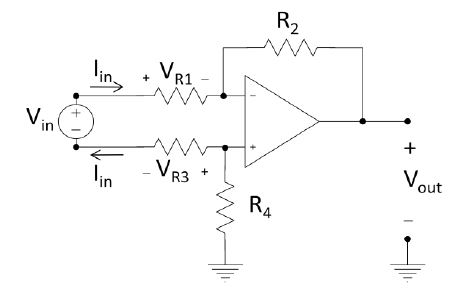
\includegraphics[width=0.5\textwidth]{billeder/Hardware/differensmodstand.JPG}
	\caption{illustration af differensforstærkerens indgangsmodstand}
	\label{fig:differensmodstand}
\end{figure}
\begin{align}
 R_{in} =V_{in}/I_{in}
 \label{eq:differensmodstand}
 \end{align}
I den ideelle verden antages det, at spændingsforskellen i mellem indgangsterminalerne er nul derfor kan der skrives vha. Kirchoffs spændingslov skrives i \ref{eq:differensmodstand2}
\begin{align}
 V_{R3}-V_{in}+V_{R1}=0=>V_{in}=V_{R3}+V_{R3}=I_{in}(R1+R3)=>R_{in}=\frac{V_{in}}{I_{in}=R1+R2}
 \label{eq:differensmodstand2}
 \end{align}
 I formel \ref{eq:differensmodstand2} vises det sig at indgangsmodstanden, er beskrevet ved modstandene i det omkring-liggende kredsløb. Dette giver anledning til at vælge så høje modstande som mulige, men store modstande øger risikoen for støj i kredsløbet. Det betyder at ønsket om en høj indgangsmodstand ikke kan opfyldes, med en simpel differensforstærker.


Punkt 3, en høj undertrykkelse af støj. Støj kan skyldes rigtig mange ting, en typisk støjkomponent er 50 Hz brum. 50 Hz brum fremkommer ofte, da støjen skyldes de omkring liggende EL installationer, hvor der foregår en elektromagnetisk kobling. Når der benyttes en differensforstærker, kan common mode støjen undertrykkes. Common mode støj er indstrålet støj der kommer på begge ledninger til differensforstærkeren. Det er differensforstærkeren god til at frasortere, fordi den trækker de to input fra hinanden. Det vil sige at den vil udligne støjen på de to ledninger, ved at subtrahere den samme værdi fra hinanden, hvilket vil give nul. En illustration af dette kan ses på figur \ref{fig:differensNoise}\citep{ASBbog}. 
\begin{figure}[H]
	\centering
	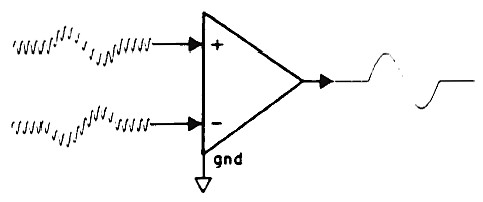
\includegraphics[width=0.5\textwidth]{billeder/Hardware/differensnoise.jpg}
	\caption{Illustration af differensforstærkerens common mode støj undertrykkelse}
	\label{fig:differensNoise}
\end{figure}

Punkt 4, en simpel forstærkning. Med det overstående kredsløb, kan en simpel forstærkning ikke opnås. Det kan det ikke da det kræver at R2 divideret med R1 er lig med R4 divideret med R3. Da modstandes præcision svinger indenfor tolerancer, vil $\frac{R2}{R1}$ aldrig være lig med $\frac{R4}{R3}$

For at opfylde de ønskede egenskaber skal differensforstærkeren modificeres. For at sikre en høj indgangsmodstand kan en spændingsfølger benyttes, som har til formål at forstærke en-til-en. Det vil sige at den i teorien har samme udgangsspænding som indgangsspændingen. se figur \ref{fig:bufferamp} for en illustration, denne sættes på begge outputs fra vægtcellen.
\begin{figure}[H]
	\centering
	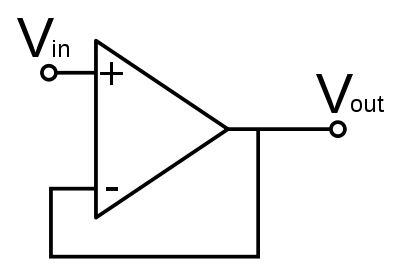
\includegraphics[width=0.5\textwidth]{billeder/Hardware/bufferamp.png}
	\caption{illustration af spændingsfølger}
	\label{fig:bufferamp}
\end{figure}
Med en spændingsfølger opnås der en høj indgangsmodstand, men signalet er stadig differentielt og uden forstærkning. Derfor indsættes der 3 modstande som vist i \ref{fig:bufferampmedgain}\citep{ASBbog}s.200
\begin{figure}[H]
	\centering
	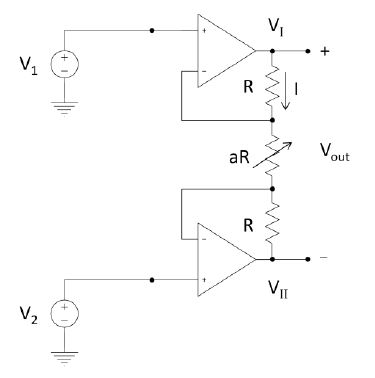
\includegraphics[width=0.5\textwidth]{billeder/Hardware/bufferampgain.JPG}
	\caption{illustration af spændingsfølger med gain}
	\label{fig:bufferampmedgain}
\end{figure}
Ved brug af KVL og KCL kan forstærkningen skrives som i \ref{eq:gain}, hvor $A_{d}$ er forstærkningen og $R_{a}$ er modstanden i midten. Dette gør forstærkningen simpel fordi der kun skal ændres en modstand. 

\begin{align}
 A_{d}=1+\frac{R+R}{R_{a}}
 \label{eq:gain}
 \end{align}
 
 Til at opfylde ønskerne om undertrykkelse af støj og et single ended output kan differensforstærkeren sættes efter spændingsfølgerne med forstærker trinet. Dermed kommer kredsløbet til at se ud som vist i figur \ref{fig:bufferampmedgaindifferens}
 
 \begin{figure}[H]
	\centering
	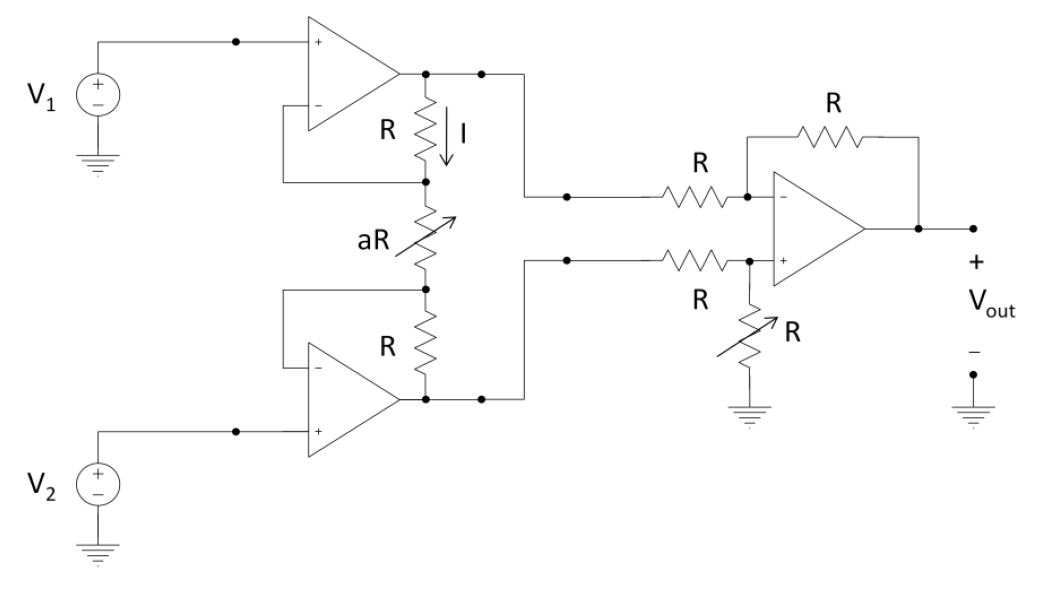
\includegraphics[width=0.5\textwidth]{billeder/Hardware/bufferampgaindifferens.JPG}
	\caption{illustration af spændingsfølger med gain og differensforstærker}
	\label{fig:bufferampmedgaindifferens}
\end{figure}

Ligning \ref{eq:instru} viser overføringsfunktionen for diagrammet i \ref{fig:bufferampmedgaindifferens}.

\begin{align}
 V_{out}=(V_{2}-V_{1})*(1+\frac{R+R}{R_{a}})
 \label{eq:instru}
 \end{align} 
 
Kredsløbet på figur \ref{fig:bufferampmedgaindifferens} kaldes en instrumentationsforstærker, hvilket der i projeket er indkøbt da den lever op til de ønskede egenskaber og er mere præcis end at lave kredsløbet selv. Den indkøbte instrumentationsforstærker hedder INA114, som har kredsløbet- og pinkonfiguration vist på figur \ref{fig:INA114diagram} og \ref{fig:INA114Pin}\ref{bilag:INA114}
 
 \begin{figure}[htbp] \centering
\begin{minipage}[b]{0.48\textwidth} \centering
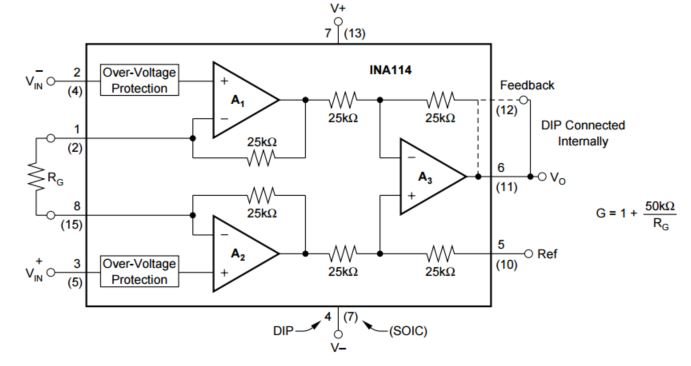
\includegraphics[width=1.00\textwidth]{billeder/Hardware/INA114diagram.JPG} % Left picture
\end{minipage} \hfill
\begin{minipage}[b]{0.48\textwidth} \centering
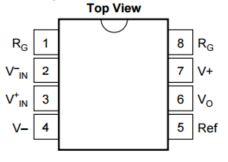
\includegraphics[width=1.00\textwidth]{billeder/Hardware/pinkonfig.JPG} % Right picture
\end{minipage} \\ % Captions og labels
\begin{minipage}[t]{0.48\textwidth}
\caption{INA114 diagram} % Left caption and label
\label{fig:INA114diagram}
\end{minipage} \hfill
\begin{minipage}[t]{0.48\textwidth}
\caption{pin konfiguration af INA114 8pin } % Right caption and label
\label{fig:INA114Pin}
\end{minipage}
\end{figure}

I databladet \ref{bilag:INA114} til INA114 ses det at den har en CMRR på 115dB, ved et gain på 1000 og en indgangsmodstand på 10G$\Omega$. Forstærkningen kan regnes ud fra formlen i databladet \ref{eq:gainina1}
\begin{align}
 G=(1+\frac{50K\Omega}{R_{G}})
 \label{eq:gainina1}
 \end{align} 
 I dette projekt skal der bruges et gain på $\frac{4,9V}{5mV}=980$, 4,9V for ikke at komme i mætning på arduinoens ADC og 5mV da det er den maksimale spænding vægtcellen kan give, ved 5V forsyning.
 \begin{align}
 R_{G}=\frac{50K\Omega}{980-1}=51\Omega
 \label{eq:gainina2}
 \end{align}
Med et gain på 980 giver en $NY_{Maksimalespænding}=980*5mV=4,9V \pm0,147V$, dvs at der nu er en opløsning på
\begin{align}
 \frac{1000g}{trin}=\frac{1000g}{1024}=0,977g/trin=>0,977*\frac{1024}{5V}=200g/V \pm30g
 \label{eq:gainina3}
 \end{align}
 
 Kredsløbet for INA114 og vægtcellen til arduinoen kan ses på figur \ref{fig:loadcelldiagram}
 
  \begin{figure}[H]
	\centering
	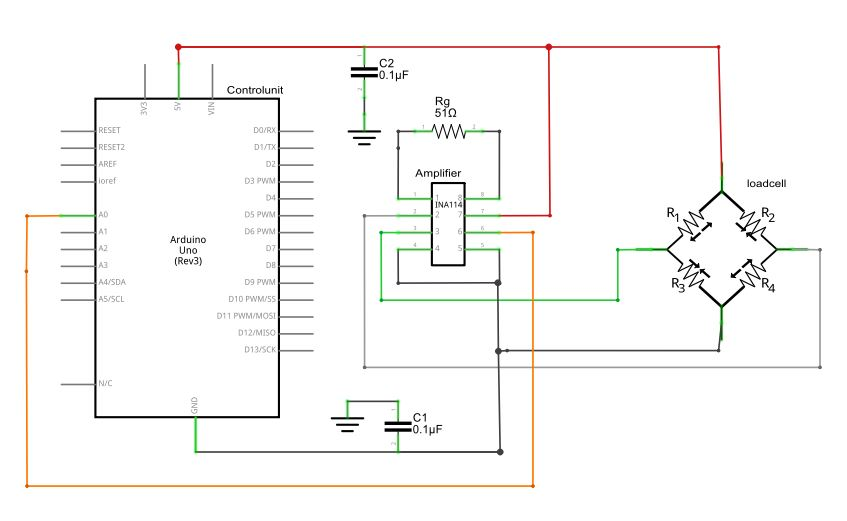
\includegraphics[width=0.9\textwidth]{billeder/Hardware/diagrammer/loadcelldiagram.JPG}
	\caption{Diagram for arduino, INA114 og vægtcelle}
	\label{fig:loadcelldiagram}
\end{figure}

%Det vil sige hvs operatøren ikke har fyldt noget i beholderen, kan der gives en systembesked omkring dette. Det mest optimale er at der hele tiden er væske i slangerne i systemet, det er det vægtcellen skal hjælpe med.

\subsection{Kameralys}
\label{subsec:kameralys}
Kameralyset skal styre lyset til kameraet, så operatøren selv kan styre hvor meget lys der skal være i kamerakammeret. Dette gøres for at få den bedste mulighed for, at detekter de langerhanske øer.
\textbf{Specifikationer for Lysdiode[\ref{bilag:L5-W55N-BVW}]:} 
\begin{center}
		\begin{longtable}{ | m{6.5cm} | m{6.5cm}| } 
			\hline
			\textbf{Specifikation} &\textbf{Værdi} \\ 
			\hline
			\textbf{Type:} & L5-w55N-BVW \\ 
			\hline
			\textbf{Anbefalet arbejdsspænding} & 3.2-3.5V \\ 
			\hline
			\textbf{Max strøm} & 100mA v. 10$\%$ duty cyklus \\ 
			\hline
			\textbf{Farve} & 6500K \\ 
			\hline
			\textbf{Lysstyrke} & 22000-33000 mcd \\ 
			\hline
			\textbf{Spredningsvinkel} & $15^{\circ}$ \\ 
			\hline
		\end{longtable}
\end{center}

Lysdioden har et tilladt strøm til Duty cyklus forhold, som kan ses på figur \ref{fig:LED1} yderligere har lysdioden også et lysintensitet til strøm forhold, dette kan ses på figur \ref{fig:LED2} 

\begin{figure}[htbp] \centering
\begin{minipage}[b]{0.48\textwidth} \centering
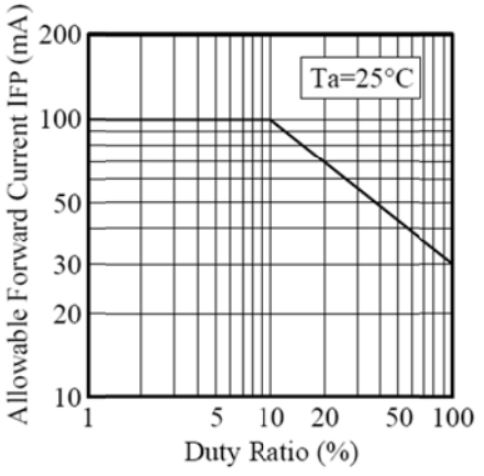
\includegraphics[width=1.00\textwidth]{billeder/Hardware/LEDDCforhold.JPG} % Left picture
\end{minipage} \hfill
\begin{minipage}[b]{0.48\textwidth} \centering
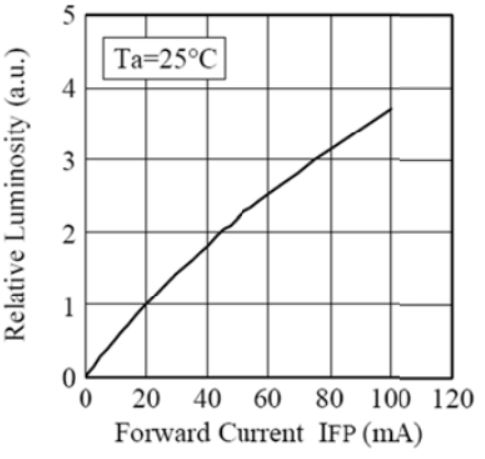
\includegraphics[width=1.00\textwidth]{billeder/Hardware/LEDlyscforhold.JPG} % Right picture
\end{minipage} \\ % Captions og labels
\begin{minipage}[t]{0.48\textwidth}
\caption{Tilladte strøm og duty cyklus forhold} % Left caption and label
\label{fig:LED1}
\end{minipage} \hfill
\begin{minipage}[t]{0.48\textwidth}
\caption{Lysintensitet og strøm forhold} % Right caption and label
\label{fig:LED2}
\end{minipage}
\end{figure}

 Kameralyset skal kunne variere, da operatøren skal kunne indstille lyset for den bedst mulige opsætning. Det gøres for at kameraet har de bedste muligheder for at detekterer de langerhanske øer. Der skal sættes 4 lysdioder i en kasse, hvor kun kameralyset lyser kassen op. Kameraet skal detektere de langerhanske øer der løber i slangen inde i kassen. Lyset implementeres for at styre lysniveauet på billederne. Da der ikke kan trækkes strøm nok ud af arduinoen, kræves det en anden forsyning til lysdioderne. Dertil udnyttes den sidste udgang i motordriveren, men da denne forsynings med 12V og lysdioder kun tåler 3.2V skal spændingen nedjusteres. Den lettest måde at gøre dette på er, at sætte lysdioderne i serie. Hvis en lysdiode bliver defekt, skabes der ingen lys til kameraet. Derfor er der valgt en løsning med modstande foran hver lysdiode. Formodstandenes værdi er beregnet ved \ref{eq:modstand}. 

\begin{align}
R=\frac{V_{source}-V_{lysdiode}}{I_{lysdiode}}=\frac{12-3.2}{20mA}=440\Omega
\label{eq:modstand}
\end{align} 
Dette giver en effekt afsætning i modstandene på $(V_{source}-V_{lysdiode}*I_{lysdiode}=8,8*20mA=0,176W)$ hvilket giver grund for at 0.33W modstande er passende.

På figur \ref{fig:LEDdiagram} vises diagrammet for Kameralyset sammen med motordriveren.
 
 \begin{figure}[H]
	\centering
	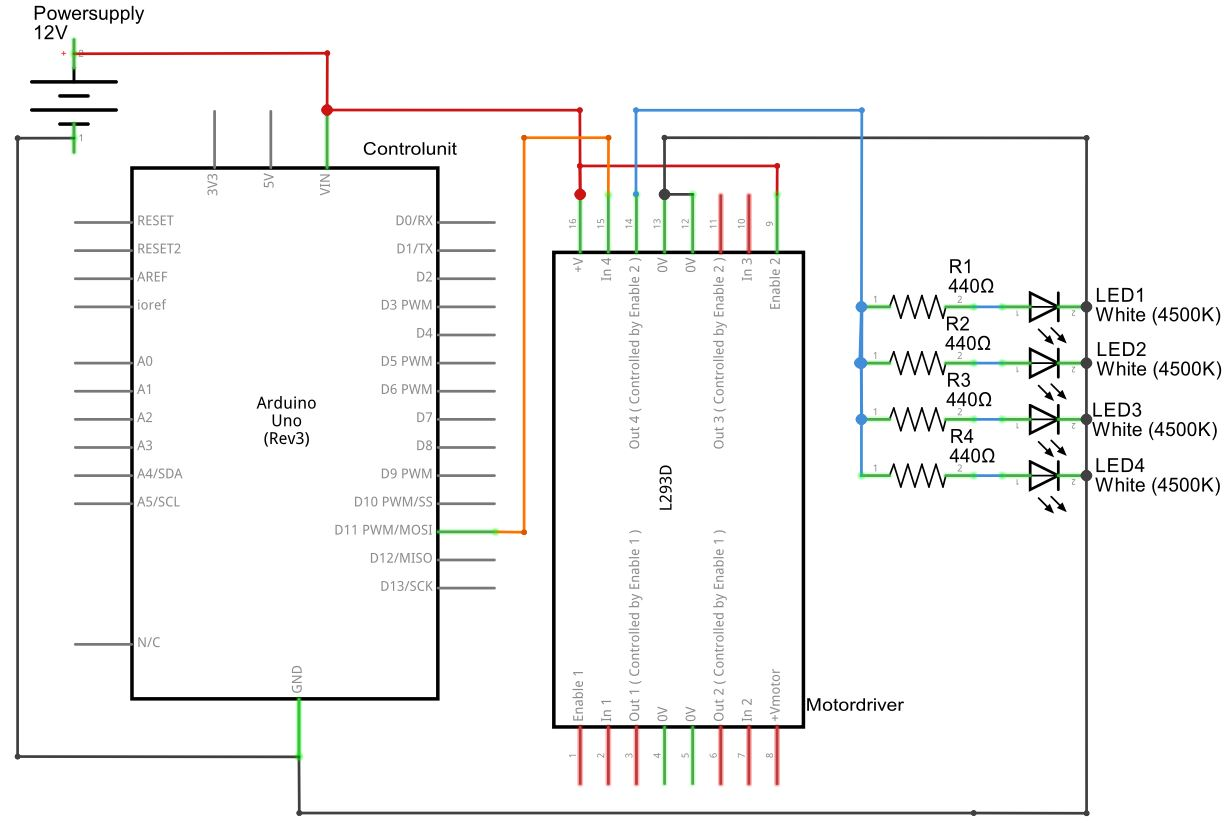
\includegraphics[width=1\textwidth]{billeder/Hardware/diagrammer/LEDdiagram.JPG}
	\caption{Kredsløbsdiagram for kameralys}
	\label{fig:LEDdiagram}
\end{figure} 


\newpage
\subsection{Beholdere}
Systemet består af tre beholdere der hver i især har sin egen funktion. Den første kaldes \textit{celleopløsningbeholderen}, som skal indeholde den usorteret opløsning med de langerhanske øer. Beholder nummer to kaldes \textit{isolerede beholderen}, som er den beholder hvor de isolerede langerhanske øer samles i. Den tredje beholder er \textit{waste beholderen}, den skal have resten af opløsningen som ikke består af langerhanske øer.
\begin{center}
		\begin{longtable}{ | m{6.5cm} | m{6.5cm}| } 
			\hline
			\textbf{Specifikation} &\textbf{Værdi} \\ 
			\hline
			\textbf{Type:} & Opløsningsbeholder(Mikrolab 33184) \\ 
			\hline
			\textbf{Størrelse:} & 250 ml \\ 
			\hline
		\end{longtable}
\end{center}
Størrelses kravene til beholderne er at opløsningsbeholderen skal mindst være 250ml, da det er den største mængde opløsning der vil blive brugt(\textit{jf. Søren Gregersen}). Wastebeholderen skal således være dobbelt så stor, så der kan gennemløbes to sorterings cyklusser uden at skulle tømme beholderen i mellem. Den isolerede beholder, skal kunne rumme mængden af de isolerede øer. Da projektet som tidligere nævnt er et ”proof of concept” er den eneste beholder der er hentet informationer om opløsningsbeholderen. Den bør være støvtæt, uden at være lufttæt da der ellers vil dannes et vakuum i beholderen. Derudover vil det være en fordel hvis den er forholdsvis robust, så den kan køles ned osv. på et senere tidspunkt. ML 33184 fås med et skruelåg med forskruninger, der kan tilpasses de indkøbte slanger. Yderligere fås den et luftfilter, så der ikke dannes vakuum i beholderen.

\subsection{Slanger}
Slangerne anvendes til at føre opløsningen med de langerhanske øer, i gennem systemet bl.a. forbi kameraet.

\textbf{Specifikationer for slangerne:(flere)} \fxnote{Tjek lige op på det her}
\begin{center}
		\begin{longtable}{ | m{6.5cm} | m{6.5cm}| } 
			\hline
			\textbf{Specifikation} &\textbf{Værdi} \\ 
			\hline
			\textbf{Materiale:} & Teflon, silikone og PVC \\ 
			\hline
			\textbf{Ydre diameter:} & ?mm  \\ 
			\hline
			\textbf{Indre diameter:} & \SI{500}{\micro\metre}-\SI{700}{\micro\metre}  \\ 
			\hline			
		\end{longtable}
\end{center}

Da de største langerhanske øer, som systemet skal håndtere er \SI{300}{\micro\metre} i diameter, derfor er det valgt at slangerne skal have en indre diameter på \SI{500}{\micro\metre}. Da det er optimalt at kameraet kan se direkte igennem slangen, er der valgt et gennemsigtigt materiale. Yderdiameteren er valgt for at, pumpen ikke skal ødelægge celler og slange, hvilket også har været med til at bestemme materialet af slangerne. 

\subsection{Glasrør}
For at sikre, at kameraet er i stand til at se de langerhanske øer, er der valgt et glasrør.

\textbf{Specifikationer for Glasrøret:} 

\begin{center}
		\begin{longtable}{ | m{6.5cm} | m{6.5cm}| } 
			\hline
			\textbf{Specifikation} &\textbf{Værdi} \\ 
			\hline
			\textbf{Materiale:} & glas \\ 
			\hline
			\textbf{Ydre diameter:} & ?mm \fxnote{Tjek lige op på det her}  \\ 
			\hline
			\textbf{Indre diameter:} & \SI{500}{\micro\metre}-\SI{700}{\micro\metre}  \\ 
			\hline			
		\end{longtable}
\end{center}

Glasrøret er tiltænkt kun til at sidde, hvor kameraet skal detektere de langerhanske øer. For at være sikker på at kameraet kan se dem. Glasrøret der er valgt er rundt. Krumningen i røret kan muligvis ændre billedet fra kameraet. Et rektangel glasrør har været overvejet, men risikoen for at de langerhanske øer kan overhale hinanden inden i er for stor. Derfor er et rundt glasrør valgt.





